\documentclass[12pt,]{book}
\usepackage{lmodern}
\usepackage{amssymb,amsmath}
\usepackage{ifxetex,ifluatex}
\usepackage{fixltx2e} % provides \textsubscript
\ifnum 0\ifxetex 1\fi\ifluatex 1\fi=0 % if pdftex
  \usepackage[T1]{fontenc}
  \usepackage[utf8]{inputenc}
\else % if luatex or xelatex
  \ifxetex
    \usepackage{mathspec}
  \else
    \usepackage{fontspec}
  \fi
  \defaultfontfeatures{Ligatures=TeX,Scale=MatchLowercase}
\fi
% use upquote if available, for straight quotes in verbatim environments
\IfFileExists{upquote.sty}{\usepackage{upquote}}{}
% use microtype if available
\IfFileExists{microtype.sty}{%
\usepackage{microtype}
\UseMicrotypeSet[protrusion]{basicmath} % disable protrusion for tt fonts
}{}
\usepackage[margin=1in]{geometry}
\usepackage{hyperref}
\hypersetup{unicode=true,
            pdftitle={Practical Data Analysis for Political Scientists},
            pdfauthor={Brenton Kenkel},
            pdfborder={0 0 0},
            breaklinks=true}
\urlstyle{same}  % don't use monospace font for urls
\usepackage{natbib}
\bibliographystyle{apalike}
\usepackage{color}
\usepackage{fancyvrb}
\newcommand{\VerbBar}{|}
\newcommand{\VERB}{\Verb[commandchars=\\\{\}]}
\DefineVerbatimEnvironment{Highlighting}{Verbatim}{commandchars=\\\{\}}
% Add ',fontsize=\small' for more characters per line
\usepackage{framed}
\definecolor{shadecolor}{RGB}{248,248,248}
\newenvironment{Shaded}{\begin{snugshade}}{\end{snugshade}}
\newcommand{\KeywordTok}[1]{\textcolor[rgb]{0.13,0.29,0.53}{\textbf{{#1}}}}
\newcommand{\DataTypeTok}[1]{\textcolor[rgb]{0.13,0.29,0.53}{{#1}}}
\newcommand{\DecValTok}[1]{\textcolor[rgb]{0.00,0.00,0.81}{{#1}}}
\newcommand{\BaseNTok}[1]{\textcolor[rgb]{0.00,0.00,0.81}{{#1}}}
\newcommand{\FloatTok}[1]{\textcolor[rgb]{0.00,0.00,0.81}{{#1}}}
\newcommand{\ConstantTok}[1]{\textcolor[rgb]{0.00,0.00,0.00}{{#1}}}
\newcommand{\CharTok}[1]{\textcolor[rgb]{0.31,0.60,0.02}{{#1}}}
\newcommand{\SpecialCharTok}[1]{\textcolor[rgb]{0.00,0.00,0.00}{{#1}}}
\newcommand{\StringTok}[1]{\textcolor[rgb]{0.31,0.60,0.02}{{#1}}}
\newcommand{\VerbatimStringTok}[1]{\textcolor[rgb]{0.31,0.60,0.02}{{#1}}}
\newcommand{\SpecialStringTok}[1]{\textcolor[rgb]{0.31,0.60,0.02}{{#1}}}
\newcommand{\ImportTok}[1]{{#1}}
\newcommand{\CommentTok}[1]{\textcolor[rgb]{0.56,0.35,0.01}{\textit{{#1}}}}
\newcommand{\DocumentationTok}[1]{\textcolor[rgb]{0.56,0.35,0.01}{\textbf{\textit{{#1}}}}}
\newcommand{\AnnotationTok}[1]{\textcolor[rgb]{0.56,0.35,0.01}{\textbf{\textit{{#1}}}}}
\newcommand{\CommentVarTok}[1]{\textcolor[rgb]{0.56,0.35,0.01}{\textbf{\textit{{#1}}}}}
\newcommand{\OtherTok}[1]{\textcolor[rgb]{0.56,0.35,0.01}{{#1}}}
\newcommand{\FunctionTok}[1]{\textcolor[rgb]{0.00,0.00,0.00}{{#1}}}
\newcommand{\VariableTok}[1]{\textcolor[rgb]{0.00,0.00,0.00}{{#1}}}
\newcommand{\ControlFlowTok}[1]{\textcolor[rgb]{0.13,0.29,0.53}{\textbf{{#1}}}}
\newcommand{\OperatorTok}[1]{\textcolor[rgb]{0.81,0.36,0.00}{\textbf{{#1}}}}
\newcommand{\BuiltInTok}[1]{{#1}}
\newcommand{\ExtensionTok}[1]{{#1}}
\newcommand{\PreprocessorTok}[1]{\textcolor[rgb]{0.56,0.35,0.01}{\textit{{#1}}}}
\newcommand{\AttributeTok}[1]{\textcolor[rgb]{0.77,0.63,0.00}{{#1}}}
\newcommand{\RegionMarkerTok}[1]{{#1}}
\newcommand{\InformationTok}[1]{\textcolor[rgb]{0.56,0.35,0.01}{\textbf{\textit{{#1}}}}}
\newcommand{\WarningTok}[1]{\textcolor[rgb]{0.56,0.35,0.01}{\textbf{\textit{{#1}}}}}
\newcommand{\AlertTok}[1]{\textcolor[rgb]{0.94,0.16,0.16}{{#1}}}
\newcommand{\ErrorTok}[1]{\textcolor[rgb]{0.64,0.00,0.00}{\textbf{{#1}}}}
\newcommand{\NormalTok}[1]{{#1}}
\usepackage{longtable,booktabs}
\usepackage{graphicx,grffile}
\makeatletter
\def\maxwidth{\ifdim\Gin@nat@width>\linewidth\linewidth\else\Gin@nat@width\fi}
\def\maxheight{\ifdim\Gin@nat@height>\textheight\textheight\else\Gin@nat@height\fi}
\makeatother
% Scale images if necessary, so that they will not overflow the page
% margins by default, and it is still possible to overwrite the defaults
% using explicit options in \includegraphics[width, height, ...]{}
\setkeys{Gin}{width=\maxwidth,height=\maxheight,keepaspectratio}
\IfFileExists{parskip.sty}{%
\usepackage{parskip}
}{% else
\setlength{\parindent}{0pt}
\setlength{\parskip}{6pt plus 2pt minus 1pt}
}
\setlength{\emergencystretch}{3em}  % prevent overfull lines
\providecommand{\tightlist}{%
  \setlength{\itemsep}{0pt}\setlength{\parskip}{0pt}}
\setcounter{secnumdepth}{5}
% Redefines (sub)paragraphs to behave more like sections
\ifx\paragraph\undefined\else
\let\oldparagraph\paragraph
\renewcommand{\paragraph}[1]{\oldparagraph{#1}\mbox{}}
\fi
\ifx\subparagraph\undefined\else
\let\oldsubparagraph\subparagraph
\renewcommand{\subparagraph}[1]{\oldsubparagraph{#1}\mbox{}}
\fi

%%% Use protect on footnotes to avoid problems with footnotes in titles
\let\rmarkdownfootnote\footnote%
\def\footnote{\protect\rmarkdownfootnote}

%%% Change title format to be more compact
\usepackage{titling}

% Create subtitle command for use in maketitle
\newcommand{\subtitle}[1]{
  \posttitle{
    \begin{center}\large#1\end{center}
    }
}

\setlength{\droptitle}{-2em}
  \title{Practical Data Analysis for Political Scientists}
  \pretitle{\vspace{\droptitle}\centering\huge}
  \posttitle{\par}
  \author{Brenton Kenkel}
  \preauthor{\centering\large\emph}
  \postauthor{\par}
  \predate{\centering\large\emph}
  \postdate{\par}
  \date{2017-01-12}

\usepackage{booktabs}

\begin{document}
\maketitle

{
\setcounter{tocdepth}{1}
\tableofcontents
}
\chapter{About This Book}\label{about-this-book}

This book contains the course notes for
\href{http://bkenkel.com}{Brenton Kenkel}'s course Statistics for
Political Research II (PSCI 8357 at Vanderbilt University). It covers
the basics of statistical modeling and programming with linear models,
along with applications in R.

This book is written in \href{http://rmarkdown.rstudio.com}{R Markdown}
and published via \href{https://bookdown.org}{Bookdown} on
\href{https://pages.github.com}{GitHub Pages}. You can find the R
Markdown source files at \url{https://github.com/brentonk/pdaps}.

This work is licensed under a
\href{http://creativecommons.org/licenses/by-nc-sa/4.0/}{Creative
Commons Attribution-NonCommercial-ShareAlike 4.0 International License}.

\chapter{Principles of Programming}\label{principles}

It may seem strange to begin a statistics class with two weeks on
programming. It is strange. Here is why I have made this strange choice.

First, as a working social scientist, most of the time you spend on data
analysis won't be on the \emph{analysis} part. It'll be on obtaining and
cleaning the data, to get it in a form that makes sense to analyze. Good
programming skills will let you spend less time cleaning data and more
time publishing papers.

Second, even if you don't want to develop good programming habits,
journals are going to force you to. Every reputable political science
journal requires that you provide replication scripts, and some of the
best (e.g., \emph{American Journal of Political Science}) have begun
auditing the replication materials as a condition of publication. Better
to learn The Right Way now when you have lots of time than to be forced
to when you're writing a dissertation or on the market or teaching your
own courses.

Third, while I feel embarrassed to invoke the cliché that is Big Data,
that doesn't mean it's not a real thing. Political scientists have
access to more data and more computing power than ever before. You can't
collect, manage, clean, and analyze large quantities of data without
understanding the basic principles of programming.

As \citet{Bowers:2011ua} puts it, ``Data analysis is computer
programming.'' By getting a PhD in political science,\footnote{Or
  whatever other social science field.} by necessity you're going to
become a computer programmer. The choice before you is whether to be a
good one or a bad one.

\citet{Wilson:2014ck} list eight ``best practices for scientific
computing.'' The first two encapsulate most of what you need to know:

\begin{enumerate}
\def\labelenumi{\arabic{enumi}.}
\tightlist
\item
  Write programs for people, not computers.
\item
  Let the computer do the work.
\end{enumerate}

\section{Write Programs for People, Not
Computers}\label{write-programs-for-people-not-computers}

The first two words here---\emph{write programs}---are crucial. When you
are doing analysis for a research project, you should be writing and
running scripts, not typing commands into the R (or Stata) console. The
console is ephemeral, but scripts are forever, at least if you save
them.

Like the manuscripts you will write to describe your findings, your
analysis scripts are a form of scientific communication. You wouldn't
write a paper that is disorganized, riddled with grammatical errors, or
incomprehensible to anyone besides yourself. Don't write your analysis
scripts that way either.

Each script should be self-contained, ideally accomplishing one major
task. Using an omnibus script that runs every bit of analysis is like
writing a paper without paragraph breaks. A typical breakdown of scripts
for a project of mine looks like:

\begin{itemize}
\tightlist
\item
  \texttt{0-download.r}: downloads the data
\item
  \texttt{1-clean.r}: cleans the data
\item
  \texttt{2-run.r}: runs the main analysis
\item
  \texttt{3-figs.r}: generates figures
\end{itemize}

The exact structure varies depending on the nature of the project.
Notice that the scripts are numbered in the order they should be run.

Within each script, write the code to make it as easy as possible for
your reader to follow what you're doing. You should indent your code
according to style conventions such as
\url{http://adv-r.had.co.nz/Style.html}. Even better, use the
\texttt{Code\ -\textgreater{}\ Reindent\ Lines} menu option in R Studio
to automatically indent according to a sane style.

\begin{Shaded}
\begin{Highlighting}[]
\CommentTok{# Bad}
\NormalTok{my_results <-}\StringTok{ }\KeywordTok{c}\NormalTok{(}\KeywordTok{mean}\NormalTok{(variable),}
\KeywordTok{quantile}\NormalTok{(variable,}
\DataTypeTok{probs =} \FloatTok{0.25}\NormalTok{),}
\KeywordTok{max}\NormalTok{(variable))}

\CommentTok{# Better}
\NormalTok{my_results <-}\StringTok{ }\KeywordTok{c}\NormalTok{(}\KeywordTok{mean}\NormalTok{(variable),}
                \KeywordTok{quantile}\NormalTok{(variable,}
                         \DataTypeTok{probs =} \FloatTok{0.25}\NormalTok{),}
                \KeywordTok{max}\NormalTok{(variable))}
\end{Highlighting}
\end{Shaded}

Another way to make your code readable---one that, unfortunately, cannot
be accomplished quite so algorithmically---is to add explanatory
comments. The point of comments is not to document how the language
works. The following comment is an extreme example of a useless comment.

\begin{Shaded}
\begin{Highlighting}[]
\CommentTok{# Take the square root of the errors and assign them to}
\CommentTok{# the output variable}
\NormalTok{output <-}\StringTok{ }\KeywordTok{sqrt}\NormalTok{(errors)}
\end{Highlighting}
\end{Shaded}

A better use for the comment would be to explain \emph{why} you're
taking the square root of the errors, at least if your purpose in doing
so would be unclear to a hypothetical reader of the code.

My basic heuristic for code readability is \emph{If I got hit by a bus
tomorrow, could one of my coauthors figure out what the hell I was doing
and finish the paper?}

\section{Let the Computer Do the
Work}\label{let-the-computer-do-the-work}

Computers are really good at structured, repetitive tasks. If you ever
find yourself entering the same thing into the computer over and over
again, you are Doing It Wrong. Your job as the human directing the
computer is to figure out the structure that underlies the repeated task
and to program the computer to do the repetition.

For example, imagine you have just run a large experiment and you want
to estimate effects by subgroups.\footnote{There could be statistical
  problems with this kind of analysis, at least if the subgroups were
  specified \emph{post hoc}. See \url{https://xkcd.com/882/}
  (``Significant''). We're going to leave this issue aside for now, but
  we'll return to it later when we discuss the statistical crisis in
  science.} Your respondents differ across four variables---party ID (R
or D), gender (male or female), race (white or nonwhite), and education
(college degree or not)---giving you 16 subgroups. You \emph{could} copy
and paste your code to estimate the treatment effect 16 times. But this
is a bad idea for a few reasons.

\begin{itemize}
\item
  Copy-paste doesn't scale. Copy-paste is managable (albeit misguided)
  for 16 iterations, but probably not for 50 and definitely not for more
  than 100.
\item
  Making changes becomes painful. Suppose you decide to change how you
  calculate the estimate. Now you have to go back and individually edit
  16 chunks of code.
\item
  Copy-paste is error-prone, and insidiously so. If you do the
  calculation wrong all 16 times, you'll probably notice. But what if
  you screwed up for just one or two cases? Are you \emph{really} going
  to go through and check that you did everything right in each
  individual case?
\end{itemize}

We're going to look at the most basic ways to get the computer to repeat
structured tasks---functions and control flow statements. To illustrate
these, we will use a result you discussed in Stat I: the central limit
theorem.

The central limit theorem concerns the \emph{sampling distribution} of
the sample mean,

\begin{equation*}
\bar{X} = \frac{1}{N} \sum_{n = 1}^{N} X_n,
\end{equation*}

where each \(X_n\) is independent and identically distributed with mean
\(\mu\) and variance \(\sigma^2\). Loosely speaking, the CLT says that
as \(N\) grows large, the sampling distribution of \(\bar{X}\) becomes
approximately normal with mean \(\mu\) and variance \(\sigma^2 / N\).

Here's what we would need to do to see the CLT in practice. We'd want to
take a bunch of samples, each of size \(N\), and calculate the sample
mean of each. Then we'd have a sample of sample means, and we could
check to verify that they are approximately normally distributed with
mean \(\mu\) and variance \(\sigma^2 / N\). This is a structured,
repetitive task---exactly the kind of thing that should be programmed.
We'll try it out with a random variable from a Poisson distribution with
\(\lambda = 3\), which has mean \(\mu = 3\) and variance
\(\sigma^2 = 3\).

First things first. We can use the \texttt{rpois} function to draw a
random sample of \(N\) numbers from the Poisson distribution.

\begin{Shaded}
\begin{Highlighting}[]
\NormalTok{samp <-}\StringTok{ }\KeywordTok{rpois}\NormalTok{(}\DecValTok{10}\NormalTok{, }\DataTypeTok{lambda =} \DecValTok{3}\NormalTok{)}
\NormalTok{samp}
\end{Highlighting}
\end{Shaded}

\begin{verbatim}
##  [1] 2 3 8 3 5 4 3 4 2 2
\end{verbatim}

To calculate the sample mean, we simply use the \texttt{mean} function.

\begin{Shaded}
\begin{Highlighting}[]
\KeywordTok{mean}\NormalTok{(samp)}
\end{Highlighting}
\end{Shaded}

\begin{verbatim}
## [1] 3.6
\end{verbatim}

We are interested in the distribution of the sample mean across many
samples like this one. To begin, we will write a \textbf{function} that
automates our core task---drawing a sample of \(N\) observations from
Poisson(3) and calculating the sample mean. A function consists of a set
of \emph{arguments} (the inputs) and a \emph{body} of code specifying
which calculations to perform on the inputs to produce the output.

\begin{Shaded}
\begin{Highlighting}[]
\NormalTok{pois_mean <-}\StringTok{ }\NormalTok{function(n_obs) \{}
  \NormalTok{samp <-}\StringTok{ }\KeywordTok{rpois}\NormalTok{(n_obs, }\DataTypeTok{lambda =} \DecValTok{3}\NormalTok{)}
  \NormalTok{ans <-}\StringTok{ }\KeywordTok{mean}\NormalTok{(samp)}
  \KeywordTok{return}\NormalTok{(ans)}
\NormalTok{\}}
\end{Highlighting}
\end{Shaded}

This code creates a function called \texttt{pois\_mean}. It has a single
argument, called \texttt{n\_obs}. It generates a random sample of
\texttt{n\_obs} draws from Poisson(3) and calculates its sample mean. It
then \texttt{return}s the sample mean as the output.

Let's try calling this function a few times, each with a sample size of
\(N = 30\). Your output will differ slightly from what's printed here,
since the function is generating random numbers.

\begin{Shaded}
\begin{Highlighting}[]
\KeywordTok{pois_mean}\NormalTok{(}\DataTypeTok{n_obs =} \DecValTok{30}\NormalTok{)}
\end{Highlighting}
\end{Shaded}

\begin{verbatim}
## [1] 3.033333
\end{verbatim}

\begin{Shaded}
\begin{Highlighting}[]
\KeywordTok{pois_mean}\NormalTok{(}\DataTypeTok{n_obs =} \DecValTok{30}\NormalTok{)}
\end{Highlighting}
\end{Shaded}

\begin{verbatim}
## [1] 2.466667
\end{verbatim}

\begin{Shaded}
\begin{Highlighting}[]
\KeywordTok{pois_mean}\NormalTok{(}\DataTypeTok{n_obs =} \DecValTok{30}\NormalTok{)}
\end{Highlighting}
\end{Shaded}

\begin{verbatim}
## [1] 2.966667
\end{verbatim}

Remember that what we're interested in is the \emph{sampling
distribution} of the sample mean---the distribution of the sample mean
across every possible sample of \(N\) observations. We can approximate
this distribution by running \texttt{pois\_mean} many times (e.g., 1000
or more). This would be infeasible via copy-paste. Instead, we will use
a \textbf{for loop}.

\begin{Shaded}
\begin{Highlighting}[]
\CommentTok{# Set up a vector to store the output}
\NormalTok{n_replicates <-}\StringTok{ }\DecValTok{1000}
\NormalTok{sampling_dist <-}\StringTok{ }\KeywordTok{rep}\NormalTok{(}\OtherTok{NA}\NormalTok{, n_replicates)}

\NormalTok{for (i in }\DecValTok{1}\NormalTok{:n_replicates) \{}
  \NormalTok{sampling_dist[i] <-}\StringTok{ }\KeywordTok{pois_mean}\NormalTok{(}\DataTypeTok{n_obs =} \DecValTok{30}\NormalTok{)}
\NormalTok{\}}
\end{Highlighting}
\end{Shaded}

Here's how the for loop works. We specified \texttt{i} as the name of
the index variable, with values \texttt{1:n\_replicates}. The for loop
takes each value in the sequence, assigns it to the variable \texttt{i},
runs the given expression (in this case, assigning the output of
\texttt{pois\_mean} to the \texttt{i}'th element of
\texttt{sampling\_dist}), and then moves on to the next value in
sequence, until it reaches the end.

Let's take a look at the results and compare them to our expectations.

\begin{Shaded}
\begin{Highlighting}[]
\KeywordTok{mean}\NormalTok{(sampling_dist)  }\CommentTok{# Expect 3}
\end{Highlighting}
\end{Shaded}

\begin{verbatim}
## [1] 2.995167
\end{verbatim}

\begin{Shaded}
\begin{Highlighting}[]
\KeywordTok{var}\NormalTok{(sampling_dist)  }\CommentTok{# Expect 1/10}
\end{Highlighting}
\end{Shaded}

\begin{verbatim}
## [1] 0.09694358
\end{verbatim}

\begin{Shaded}
\begin{Highlighting}[]
\KeywordTok{hist}\NormalTok{(sampling_dist)  }\CommentTok{# Expect roughly normal}
\end{Highlighting}
\end{Shaded}

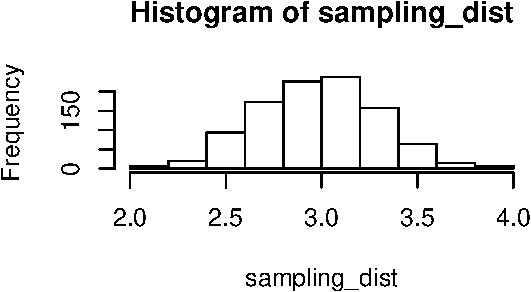
\includegraphics{bookdown-demo_files/figure-latex/sampling-dist-results-1.pdf}

For loops are fun, but don't overuse them. Many simple operations are
\textbf{vectorized} and don't require a loop. For example, suppose you
want to take the square of a sequence of numbers. You could use a for
loop \ldots{}

\begin{Shaded}
\begin{Highlighting}[]
\NormalTok{input <-}\StringTok{ }\KeywordTok{c}\NormalTok{(}\DecValTok{1}\NormalTok{, }\DecValTok{3}\NormalTok{, }\DecValTok{7}\NormalTok{, }\DecValTok{29}\NormalTok{)}
\NormalTok{output <-}\StringTok{ }\KeywordTok{rep}\NormalTok{(}\OtherTok{NA}\NormalTok{, }\KeywordTok{length}\NormalTok{(input))}

\NormalTok{for (i in }\DecValTok{1}\NormalTok{:}\KeywordTok{length}\NormalTok{(input)) \{}
  \NormalTok{output[i] <-}\StringTok{ }\NormalTok{input[i]^}\DecValTok{2}
\NormalTok{\}}

\NormalTok{output}
\end{Highlighting}
\end{Shaded}

\begin{verbatim}
## [1]   1   9  49 841
\end{verbatim}

\ldots{} but it's faster (in terms of computational speed) and easier to
just take advantage of vectorization:

\begin{Shaded}
\begin{Highlighting}[]
\NormalTok{input^}\DecValTok{2}
\end{Highlighting}
\end{Shaded}

\begin{verbatim}
## [1]   1   9  49 841
\end{verbatim}

Another useful piece of control flow is \textbf{if/else statements}.
These check a logical condition---an expression whose value is
\texttt{TRUE} or \texttt{FALSE}---and run different code depending on
the value of the expression. (You may want to catch up on the comparison
operators: \texttt{==}, \texttt{\textgreater{}},
\texttt{\textgreater{}=}, \texttt{\textless{}}, \texttt{\textless{}=},
etc.)

Let's edit the \texttt{pois\_mean} function to allow us to calculate the
median instead of the mean. We'll add a second argument to the function,
and implement the option using an if/else statement.

\begin{Shaded}
\begin{Highlighting}[]
\NormalTok{pois_mean <-}\StringTok{ }\NormalTok{function(n_obs, }\DataTypeTok{use_median =} \OtherTok{FALSE}\NormalTok{) \{}
  \NormalTok{samp <-}\StringTok{ }\KeywordTok{rpois}\NormalTok{(n_obs, }\DataTypeTok{lambda =} \DecValTok{3}\NormalTok{)}
  \NormalTok{if (use_median) \{}
    \NormalTok{ans <-}\StringTok{ }\KeywordTok{median}\NormalTok{(samp)}
  \NormalTok{\} else \{}
    \NormalTok{ans <-}\StringTok{ }\KeywordTok{mean}\NormalTok{(samp)}
  \NormalTok{\}}
  \KeywordTok{return}\NormalTok{(ans)}
\NormalTok{\}}
\end{Highlighting}
\end{Shaded}

A couple of things to notice about the structure of the function. We use
a comma to separate multiple function arguments. Also, we've specified
\texttt{FALSE} as the \emph{default} for the \texttt{use\_median}
argument. If we call the function without explicitly specifying a value
for \texttt{use\_median}, the function sets it to \texttt{FALSE}.

\begin{Shaded}
\begin{Highlighting}[]
\KeywordTok{pois_mean}\NormalTok{(}\DataTypeTok{n_obs =} \DecValTok{9}\NormalTok{)}
\end{Highlighting}
\end{Shaded}

\begin{verbatim}
## [1] 3.777778
\end{verbatim}

\begin{Shaded}
\begin{Highlighting}[]
\KeywordTok{pois_mean}\NormalTok{(}\DataTypeTok{n_obs =} \DecValTok{9}\NormalTok{, }\DataTypeTok{use_median =} \OtherTok{TRUE}\NormalTok{)}
\end{Highlighting}
\end{Shaded}

\begin{verbatim}
## [1] 2
\end{verbatim}

\begin{Shaded}
\begin{Highlighting}[]
\KeywordTok{pois_mean}\NormalTok{(}\DataTypeTok{n_obs =} \DecValTok{9}\NormalTok{, }\DataTypeTok{use_median =} \OtherTok{FALSE}\NormalTok{)}
\end{Highlighting}
\end{Shaded}

\begin{verbatim}
## [1] 2.666667
\end{verbatim}

There is a vectorized version of if/else statements called, naturally,
the \texttt{ifelse} function. This function takes three arguments, each
a vector of the same length: (1) a logical condition, (2) an output
value if the condition is \texttt{TRUE}, (3) an output value if the
condition is \texttt{FALSE}.

\begin{Shaded}
\begin{Highlighting}[]
\NormalTok{x <-}\StringTok{ }\DecValTok{1}\NormalTok{:}\DecValTok{10}
\NormalTok{big_x <-}\StringTok{ }\NormalTok{x *}\StringTok{ }\DecValTok{100}
\NormalTok{small_x <-}\StringTok{ }\NormalTok{x *}\StringTok{ }\NormalTok{-}\DecValTok{100}

\KeywordTok{ifelse}\NormalTok{(x >}\StringTok{ }\DecValTok{5}\NormalTok{, big_x, small_x)}
\end{Highlighting}
\end{Shaded}

\begin{verbatim}
##  [1] -100 -200 -300 -400 -500  600  700  800  900 1000
\end{verbatim}

Functions, for loops, and if/else statements are just a few of the
useful tools for programming in R.\footnote{Others include the
  \texttt{replicate} function, the \texttt{apply} family of functions
  (\texttt{sapply}, \texttt{lapply}, \texttt{tapply}, \texttt{mapply},
  \ldots{}), the \textbf{foreach} package, the \textbf{purrr} package,
  just to name a few of the most useful off the top of my head.} But
even these simple tools are enough to allow you to do much more at scale
than you could with a copy-paste philosophy.

\chapter{Working with Data}\label{data}

Let me repeat something I said last week. In your careers as social
scientists, starting with your dissertation research---if not
earlier---you will probably spend more time collecting, merging, and
cleaning data than you will on statistical analysis. So it's worth
taking some time to learn how to do this well.

Best practices for data management can be summarized in a single
sentence: \emph{Record and document everything you do to the data.}

The first corollary of this principle is that raw data is sacrosanct.
You should never edit raw data ``in place''. Once you download the raw
data file, that file should never change.\footnote{Even if it's data you
  collected yourself, that data should still have a ``canonical''
  representation that never gets overwritten. See \citet{Leek:2015uw}
  for more on distributing your own data.}

\bibliography{packages.bib,book.bib,psci-8357.bib}


\end{document}
